\chapter{Orbital workflow} \label{workflow}

\section{Registration} \label{registration}

To enroll in Orbital program, students will need to register in Skylab first. When a user first logs into Skylab, a \textit{User} object will be created for user. And since it is the first time the user logins to the system, there is not role belonging to current user. Then Skylab assumes that the user is trying to register and therefore a link to registration will be displayed. This workflow works for most users who are students in Orbital program. As for roles like \textit{Adviser}, \textit{Mentor} and \textit{Tutor}, admin users will create those roles manually. This is because there are only a few such roles and they have higher privileges and therefore creation of such roles should definitely be controlled by admin users.

For students` registration, after a user click the registration link a form consisting of different questions will be presented to the user. Among these questions, several are to get a sense of what sort of interests the user has for the project over the summer. The user is supposed to select interested topics from different categories like programming language, web framework or mobile platform, IDE or text editor, e-commerce, cloud platform, purpose, embedded system, game framework, content management system and audience. These information will be recorded for match-making among students who need to find a teammate in Skylab.

After completing the registration form, if the user already has a teammate in mind, he/she can send an invitation to the potential teammate to form a team. Some users, on the other hand, do not have anyone to partner with for Orbital yet and a match-making algorithm will be run offline by admin user based on the interested topics they have selected during registration. An illustration of the whole workflow is as Figure~\ref{fig:RegistrationWorkflow}.

\begin{figure}[h]
  \centering
  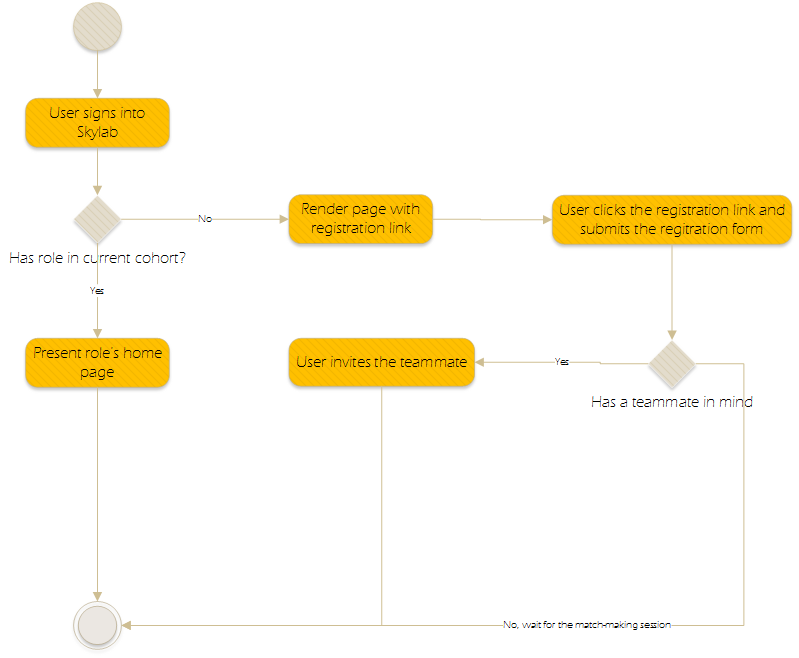
\includegraphics[width=\textwidth]{Images/Skylab_Registration_Workflow.png}
  \caption{Illustration of registration workflow in Skylab}
  \label{fig:RegistrationWorkflow}
\end{figure}

\subsection{Match making algorithm}

For students who do not have potential teammates at the time of registration, we will run a matching making algorithm based on the interested topics recorded in registration form submission. The algorithm composes of mainly two steps:

\begin{itemize}
  \item Calculate inverse document frequency of tags: inverse document frequency is to reflect how rare a term is in the corpus\cite{citationir}. In Skylab`s match making`s case, a document is a user`s selection of interested topics, or tags; the corpus is the collection of users` interested topic sets; a term is a tag in a users` selections. If a term(tag) is rare among registration form results, we will be more confident that if both students choose this term and they will have higher chance of forming a team. The formula of calculation is as Formula~\ref{eq:idf}.

  \begin{equation}
    idf(t,D) = \log \frac{N}{\{ d \in D : t \in d \} + 1} \
    \label{eq:idf}
  \end{equation}
  
  with \(N\) as total number of documents in the corpus \( N = |D| \) and \(\{ d \in D : t \in d \}\) as number of documents where the term \(t\) appears\cite{citationir}.

  \item Construct a vector space model based on students` selected tags and each tag`s weight calculated in previous step and calculate similarity(cosine) of different students. The formula for calculating cosine of two vectors is as Formula~\ref{eq:veccos}\cite{citationvecspacemodel}.

  \begin{equation}
    \cos\theta  = \frac{d_2 \cdot q}{ \norm{d_2} \norm{q} } \
    \label{eq:veccos}
  \end{equation}

  And we represent a user`s interested topics with tags` weights and the similarity between 2 users will be the cosine between 2 vectors representing the 2 users. The formula for calculating cosine of two vectors is as Formula~\ref{eq:similarity}\cite{citationvecspacemodel}.

  \begin{equation}
    sim(d_j, q)  = \frac{d_j \cdot q}{ \norm{d_j} \norm{q} } \ = \frac{sum_{i=1}^{N} \omega_{i,j} \omega_{i,q}}{ \sqrt{sum_{i=1}^{N} \omega_{i,j}^2} \sqrt{sum_{i=1}^{N} \omega_{i,q}^2}} \
    \label{eq:similarity}
  \end{equation}

\end{itemize}

As matching making only needs to be run once before Orbital officially starts for those students who do no have a team yet, the algorithm is currently designed to run offline as a rake task. Currently it is only for students but in the future with recoding of mentors` and advisers` interested tags, this algorithm can be easily extended to students and mentors or students and advisers as well.

\section{Submission} \label{submission}

Students in Orbital are supposed to report their progress regarding their project at each milestone via \textit{Submission}. Basically a submission contains 3 parts:

\begin{itemize}
  \item README: highlights what are the changes and new features in the project.
  \item Project Log: a summary of work done during the phase and time used for each task.
  \item Video link: a link to a video introducing the project to evaluators.
\end{itemize}

As the structure of \textit{README} and \textit{Project Log} is free and we should allow creativity of students when it comes to describing their own projects, we decided to support rich text for submissions and there are some issues coming along with this decision such as SQL injection and XSS attacks. What is more, during use of Skylab, many good suggestions regarding user experience were brought up by students and advisers, like uploading of images and auto-expanding textareas during editing.

\subsection{Handling of rich text}

We used TinyMCE to support rich text editing feature in Skylab as it is a very popular WYSIWYG(what-you-see-is-what-you-get) editor with a rich set of features\cite{citationtinymce}. There are some libraries with markdown syntax supported such as EpicEditor, Vue.js and Hallo.js which are more lightweight. However, as Skylab is built for freshmen to get more hands-on experience with coding, we do not expect students to be equipped with much prior knowledge such as markdown syntax. In the contrast, markup based editors such as TinyMCE and CKEditor do not require any learning and are easily to get started with. What is more, the large community using TinyMCE has made various plug-ins available for different features. There are also quite good resources online about integrating TinyMCE editor in a Rails project. Therefore, we decided to use TinyMCE for \textit{Submissions}' rich text support.

One particular disadvantage of using TinyMCE is that the size of this editor is pretty large and loading of the page will be slowed down because of it. Therefore, TinyMCE related resources is only loaded if the page is requiring rich text editing. This is done by configuration to disable auto loading of all JavaScript, which is the default behavior of Rails. In this way, most pages can be loaded within a very short time. What is more, assets whose names start with ``tinymce'' are set to expire in a year instead of the usually one week`s expiration for other assets to reduce frequent requesting of such resources from clients.

Rails has built-in checking against SQL injection attacks and therefore Skylab is safe from such attacks when storing submissions' contents\cite{citationrorsecurity}. However, there is still currently a known bug in the implementation when it comes to viewing of submissions. As contents like \textit{README} and \textit{Project Log} should be rendered as rich text, it is possible for students to perform XSS attacks by injecting executable JavaScript code in the submission. This sort of vulnerabilities will be fixed in the future.

\subsection{Usability}

Skylab is a software engineering project and therefore improvements in user experience is one key part when it comes to implementation. During the use of Skylab, many suggestions were brought up by students and advisers about usability. And by addressing these issues, Skylab is serving users better with a smoother user experience.

\subsubsection{Target Milestone Selection}

When Skylab was used for the first time, students were expected to choose the target milestone, which the submission is for. However, many students reported that it is just a redundant step as every time they will only submit to the currently active milestone. After hearing this, a quick fix of automatically selecting the current milestone for students using JavaScript functions was done, while the manual selection is still possible. And then during the \textit{Adviser Focus Group Meeting}, some advisers further pointed out that the selection should not even be presented to users as it is of completely no use and therefore the whole selection was completely removed from Skylab after the meeting by moving the task to the backend logic. 

\subsubsection{Rich Text Editing}

As quite some students want to insert image to \textit{README} sections, an image uploading feature was soon added to submission page for users' convenience. Behind the scene Skylab is using a third-party API from Imgur. This was done mainly for 2 reasons: using Imgur is relatively easy to implement; we can also avoid heavy server load due to file uploading and possible attacks in uploaded files.

Another improvement over user experience is auto expanding of TinyMCE editing area as feedback from students mentioned that their \textit{README} and \textit{Project Log} are usually quite lengthy. So auto expanding would not require too much scrolling during creating/editing a submission.

\section{Peer Evaluation} \label{peerevaluation}
 
 After students have submitted to milestones, peer evaluation process can begin. Teams will look through evaluated teams' projects and submissions and then evaluate their performance in \textit{PeerEvaluation}, which is a very important component in determining whether the evaluated teams can pass Orbital or not. Although there are different questions for each peer evaluation, all evaluations contains essentially 2 parts:

 \begin{itemize}
  \item Public: a section with general feedback on how well the evaluated team has done and the response will be viewed by target team with evaluator team name available.
  \item Private: a section with critiques and overall rating and critiques will only be viewed by target team without any evaluator team information while overall rating is only for grading purpose and not viewable by target teams.
\end{itemize}

\subsection{Loading of Peer Evaluation templates}

When Skylab was first developed, the public part of a \textit{PeerEvaluation} templates will be one html form and the private part is another one. This means all questions in the public part are coded in one predefined html template and same goes for questions in private part.

This approach does not seem to have much problem at first and it really served Skylab's purpose well by delivering perfectly workable features in time. However, since questions are different for different milestones, separate templates have to be created for each new milestone. And when user wants to view/submit/edit a \textit{PeerEvaluation}, the corresponding templates will have to be loaded based on properties of the milestone. In this way, the system is not really open to extension and clearly it violates Open-Close principle. After realizing this, a system for dynamically creating questions has been implemented for \textit{Feedback} and migration of \textit{PeerEvaluations} to the survey-template-and-questions based system has been done as well. A more detailed description for how the dynamic loading of questions is in Section~\ref{feedback}.

\section{Feedback} \label{feedback}

\textit{Feedback} is for evaluated teams to evaluate the \textit{PeerEvaluations} they have received and it is also a very important component in determining whether the evaluator team can pass or not. After realizing the lack of extensibility in the design for \textit{PeerEvaluations} and with more time available for implementation of \textit{Feedback}, a survey-template-and-questions system has been set up, which made the system open to extensions for more questions and even question types.

\subsection{Survey-template-and-questions system}

The basic flow when a request to create a \textit{Feedback} is illustrated in the Figure~\ref{fig:FeedbackFlow}:

\begin{figure}[h]
  \centering
  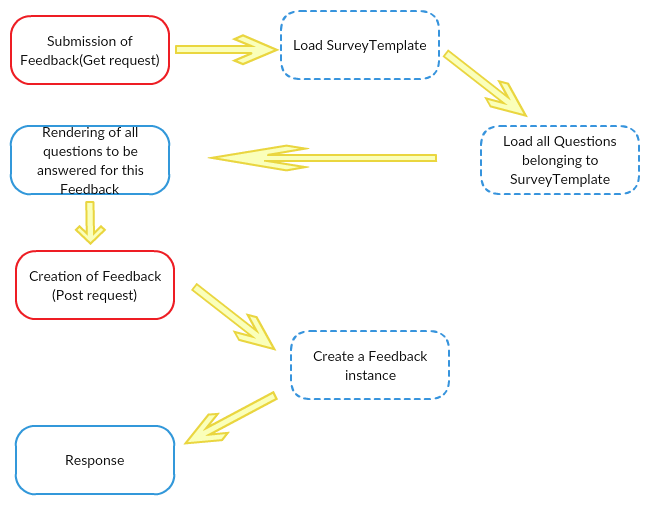
\includegraphics[width=0.8\textwidth]{Images/Skylab_Feedback_Flow.png}
  \caption{Flow of a feedback creation process}
  \label{fig:FeedbackFlow}
\end{figure}

So when a student clicks the button to create feedback, \textit{FeedbacksController}'s \textit{new} action will be invoked and inside the method, the corresponding \textit{SurveyTemplate} and all \textit{Questions} belonging to the SurveyTemplate will be sent to view. Then instruction for the \textit{Feedback} and all questions will be rendered as response to the student. After the student completed and pressed submit button, responses to all questions will be sent to server and a Feedback instance containing all submitted responses will be created.

There currently 4 types of \textit{Questions} in the system:

\begin{itemize}
  \item \textbf{TextQuestion}: a text question which will be rendered in the format of textarea and text-based responses are expected. 
  \item \textbf{RichTextQuestion}: a rich text question which will be rendered in the format of TinyMCE editable area and rich text is expected as response.
  \item \textbf{MultipleChoiceQuestion}: a multiple choice question which will be rendered as radio buttons followed by option descriptions and one option value is expected.
  \item \textbf{MultipleSelectQuestion}: a multiple choice question which will be rendered as a select with multiple enabled with each option as one choice of selection.
\end{itemize}

\begin{figure}[h]
    \centering
    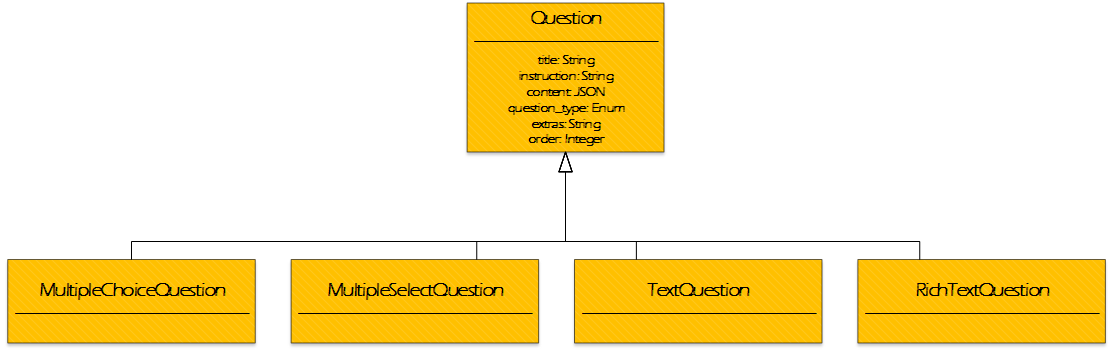
\includegraphics[width=\textwidth]{Images/Skylab_Questions.png}
    \caption{3 types of questions in Skylab}
\end{figure}

All types of question will have \textit{title}, \textit{instruction}, \textit{content}, \textit{extras} and \textit{question\_type} and each type of question will have its own way of rendering and validation. In this way, adding new types of questions can simply be done via creating a new question model with its own rendering and validation methods.
